%
% Simple Latex 2e template
%
\documentclass[12pt]{article}
\usepackage[usenames,dvips]{pstcol}
\usepackage{color}
\usepackage{amssymb}
\usepackage{epsfig}
\usepackage{footnote}
\usepackage{longtable}
\usepackage{verbatim}
\usepackage{array,multirow}
%\usepackage{titlesec}
%
% You can't use subfigure and subcaption at the same time (!)
%\usepackage{subfigure}
%\usepackage{subfigure}
% new for subfigures
\usepackage{graphicx}
\usepackage{caption}
%\usepackage{subcaption}
%
% Using .ps files with pdflatex
\usepackage{epstopdf}
% Instructions- do \includegraphics{file.eps} and then run pdflatex
%
%\usepackage{slidesec}

%\input{seminar.bug}
%\slidesmag{3}
%\usepackage[letterpaper]{geometry}
%\usepackage{fancybox}
%\usepackage{charter}
%\usepackage{feynmf}
%\usepackage{fancyhdr}
%
% make \paragraph a subsubsubsection
\setcounter{secnumdepth}{4}
%\titleformat{\paragraph}
%{\normalfont\normalsize\bfseries}{\theparagraph}{1em}{}
%\titlespacing*{\paragraph} {0pt}{3.25ex plus 1ex minus .2ex}{1.5ex plus .2ex}
%
%\include{symbols}
%
\textwidth 6.8in
\textheight 9.5in
\topmargin -0.6in
\oddsidemargin 0.0in
\evensidemargin 0.0in
\parindent 0.5in
\def\changemargin#1#2{\list{}{\rightmargin#2\leftmargin#1}\item[]}
\let\endchangemargin=\endlist 
%
\def\baselinestretch{1.0}
%
\newcommand{\smaller}{\fontsize{8}{12}\selectfont}
\newrgbcolor{maroon}{.45 0.1 0.1}
%
% Try making it behave with figures
%
\renewcommand{\topfraction}{0.85}
\renewcommand{\textfraction}{0.1}
\renewcommand{\floatpagefraction}{0.75}
%
\newcommand{\Kzero}{\mbox{$\rm K^{0}$~}}
%\newcommand{\K}{\mbox{$K$~}}
%\newcommand{\pi}{\mbox{$\pi$~}}
%
% Begin document
%

\begin{document}
\pagestyle{plain}
%\renewcommand{\headrulewidth}{0pt}
%

\begin{flushright}
Version 1.01\\
\today
\end{flushright}
%
% Title
%
\begin{center}
{\Large\bf Energy and Flavor Discrimination Using Precision Time
  Structure in On-Axis Neutrino Beams}\\

\vskip0.2in

Evan Angelico, Andrey Elagin, Jonathan Eisch, Henry J. Frisch, Sergei
  Nagaitsev, Matthew Wetstein\\

Addresses etc. (with institution assignments fixed)
\end{center}


%\address[UofC]{Enrico Fermi Institute, University of Chicago, Chicago IL 60637}
%\address[Fermilab]{Fermi National Laboratory, Batavia IL 60510}
%\address[ISU]{Matt to Fill in}


%
% Accelerator Considerations: Can One Rebunch the Protons at Higher RF Frequency?}
%
\section{Accelerator Modifications: Rebunching protons at a higher RF frequency}
\label{RF}

\subsection{Properties of the present 53.1MHz proton bunch}

\subsection{Higher frequency RF structure and hardware}

%\subsection{Other Constraints: Radiation Losses}

\subsection{Example of a rebunching procedure in the Fermilab Main Injector}

\begin{figure}[t]
	\begin{center}
        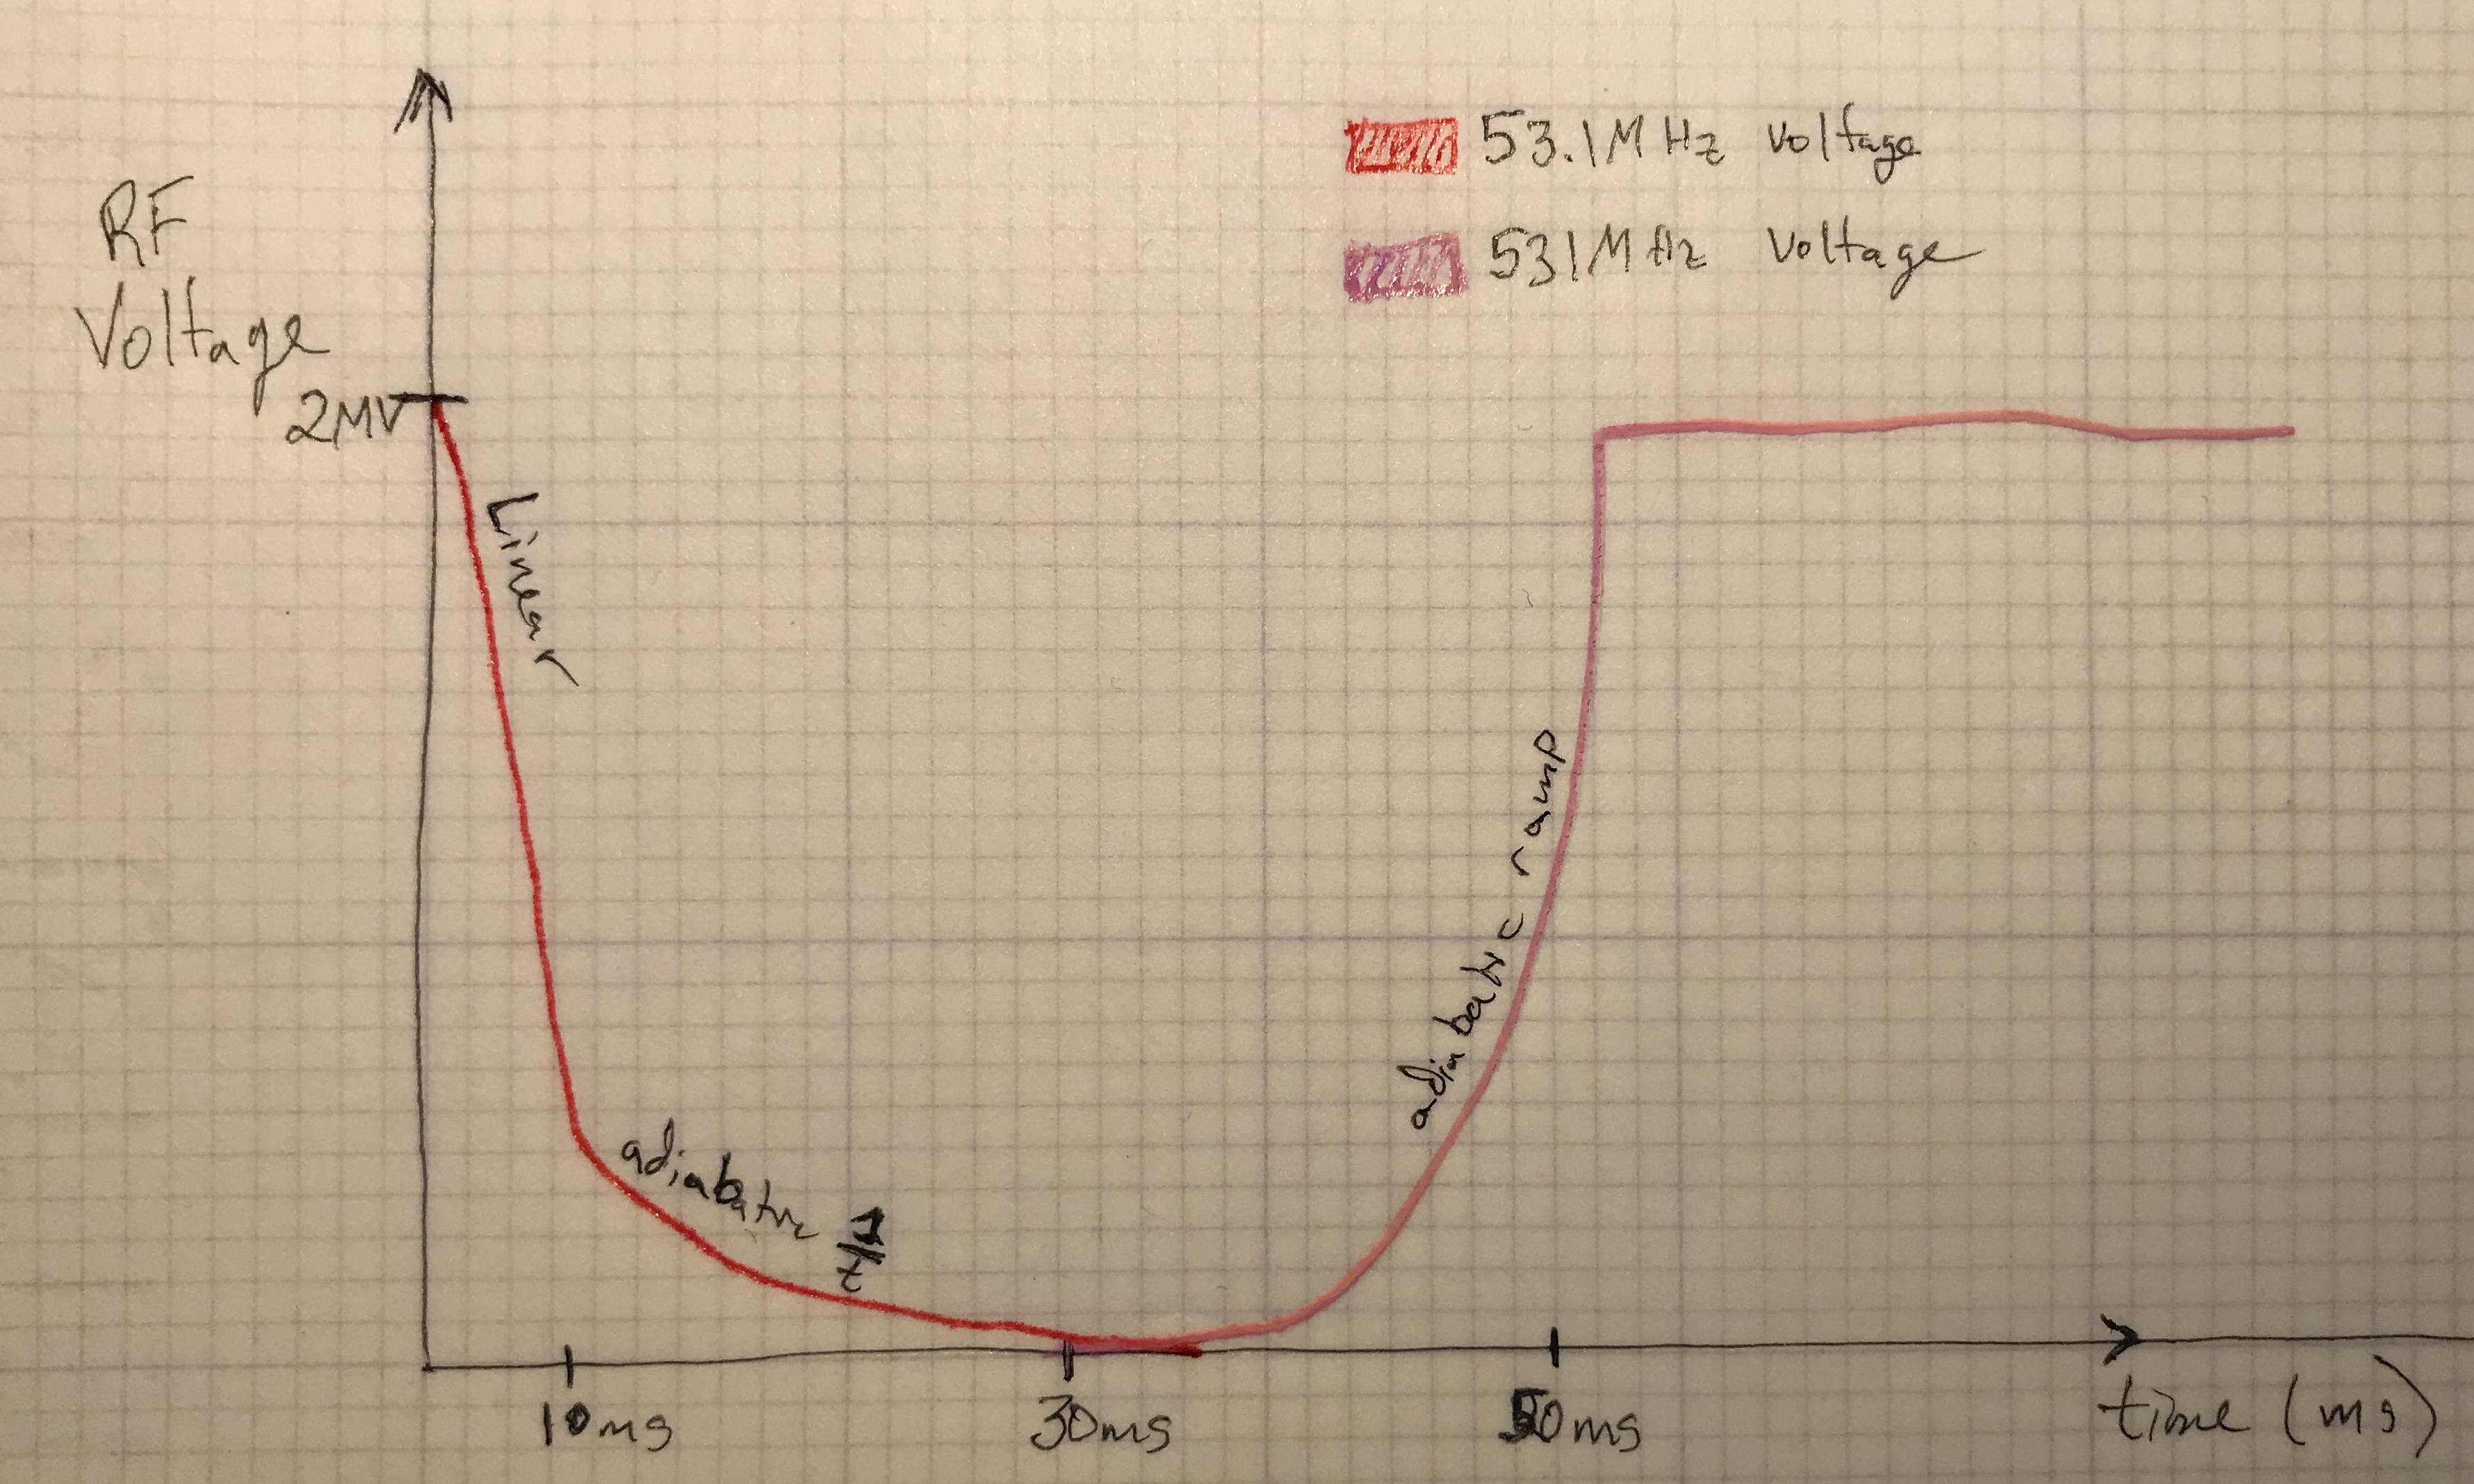
\includegraphics[width=1.0\linewidth]{Figures/draft_transition_voltages.JPG}
	\end{center}
	\caption{An example of the applied voltages to the 53.1MHz cavities (red) and the 531MHz cavity (pink). The 53.1MHz voltage function is a piece-wise function starting with linear decrease and then an adiabatic decrease using function *** down to 0 volts.}
		\label{fig:transition_voltages}
\end{figure}

\begin{figure}[t]
	\begin{center}
        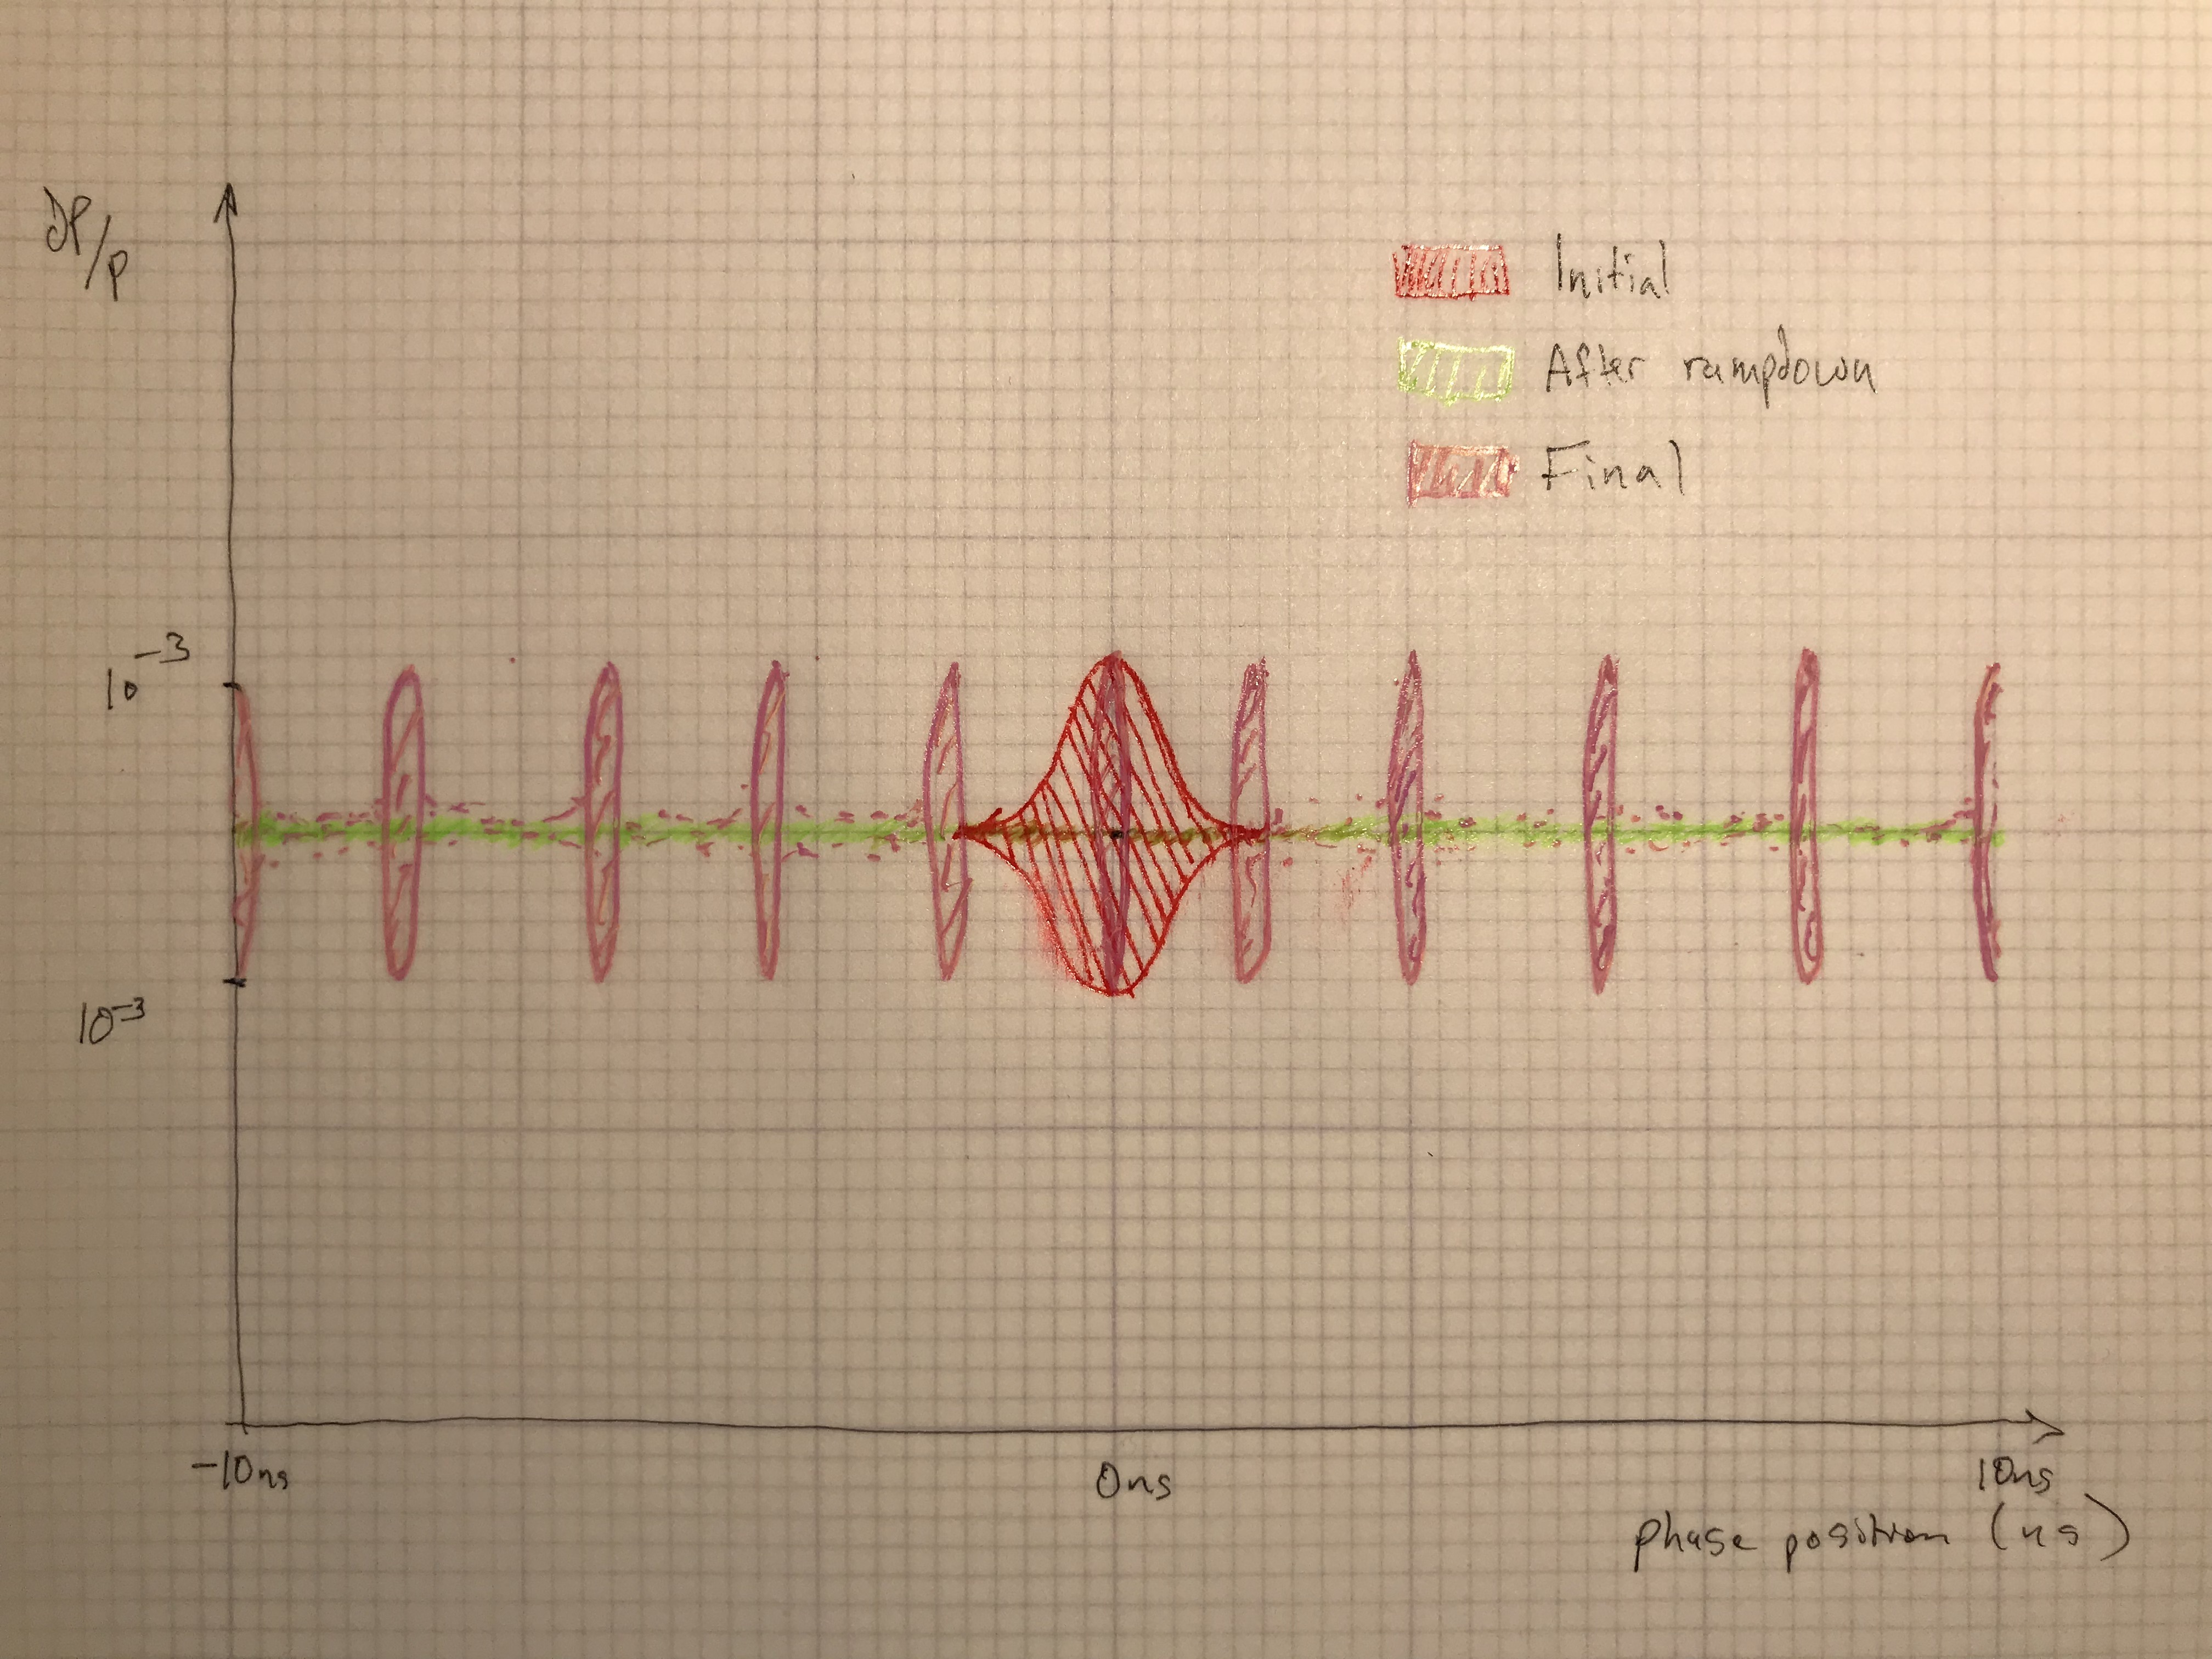
\includegraphics[width=1.0\linewidth]{Figures/draft_bunch_distributions.JPG}
	\end{center}
	\caption{Distribution of protons in energy spread vs. RF phase for the initial main injector proton bunch (red), the transition time between the two RF frequencies (green), and the end point after ramping the high frequency voltage (pink). This particular rebunching took a total of 50ms, a 4\% addition to the total cycle time.}
		\label{fig:bunch_distributions}
\end{figure}

\begin{figure}[t]
	\begin{center}
        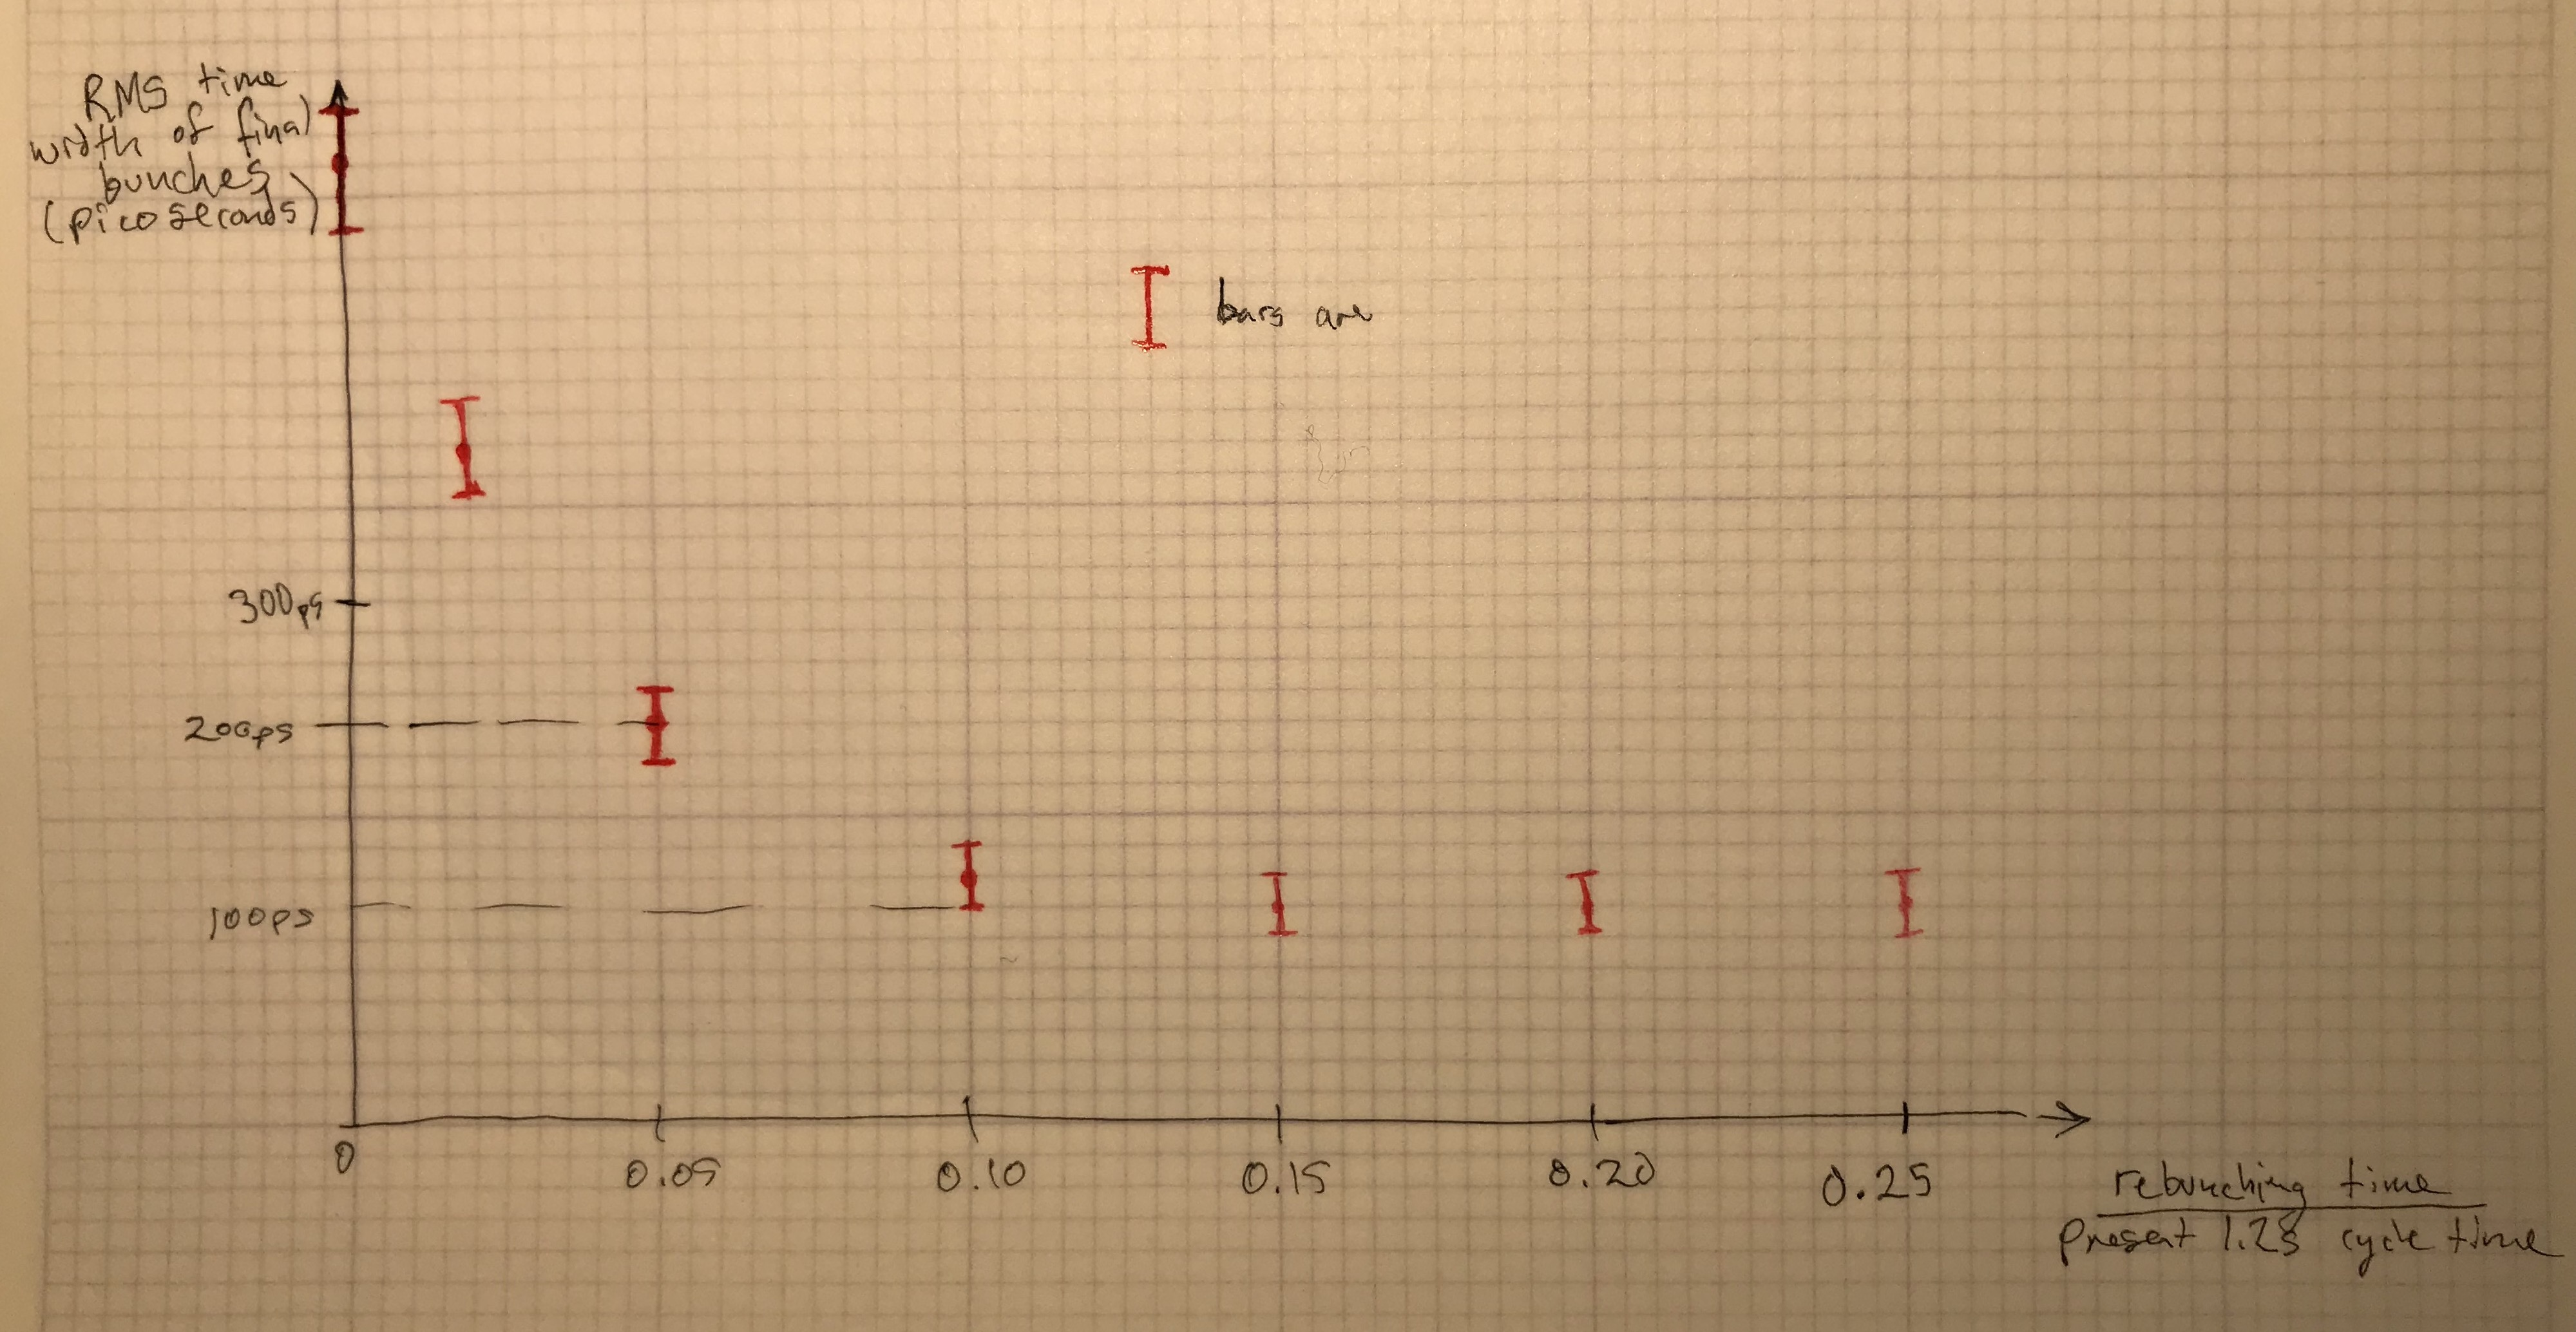
\includegraphics[width=1.0\linewidth]{Figures/draft_rms_vs_time.JPG}
	\end{center}
	\caption{The root-mean-square of the time distribution one of the thin, high-frequency bunches after going through a rebunching procedure that takes time $t$, where the x-axis is the ratio of $t$ to the present cycle time of $1.2$ seconds. Longer rebunching time corresponds to a reduction in POT because it increases the period between main injector dumps.}
		\label{fig:bunch_width_curve}
\end{figure}


\begin{thebibliography}{99}
\bibitem{bibitem} bib1 
%\bibitem{}
\end{thebibliography}

\end{document}

%%%%%%%%%%%%%%%%%%%%%%%%%%%%%%%%%%%%%%%%%%%%%%%%%%%%%%%%%%%%%%%%%%
%\section{}
%\label{}
%\subsection{}
%Section~\ref{
\begin{figure}[h]
	\begin{center}
           	\includegraphics[width=0.7 \linewidth]{Figures/}
	\end{center}
	\caption{}
	\label{fig:}
\end{figure}
